\section{Measurement Regions}%
\label{sec:Regions}

This section presents the final event selection that is applied to define the measurement phase space.
Only events passing all selection criteria are considered in the definition of the fiducial cross section.
Two analysis regions are defined and summarized in Table~\ref{tab:RegionDefinitions}.

The selection is optimised using simulated MC event samples.
All events are required to contain exactly one signal lepton as defined in ....
Prompt leptonic \( \tau \) decays are considered signal in this analysis and therefore included.
Events are selected with a single lepton trigger and a minimum \pt requirement of \qty{30}{\GeV} is placed on the lepton.
At least three jets are expected in the signal process: two $b$ jets and at least one jet from the hadronic \Wboson decay.
The neutrino from the leptonic \Wboson boson decay introduces \met.
A cut is defined on \( \met + \mtW > \qty{60}{\GeV} \) to remove background from QCD events
with a mis-identified or non-prompt lepton.
The missing transverse mass \mtW is computed from
the lepton and \met 4-vectors where the \(z\)-component is set to 0.

The \textit{Loose} region defines the most general phase space constraining the interference
effects between \ttbar and \tW processes and improve the modeling over a large kinematic region.
The explicit reconstruction of the hadronic \Wboson boson introduced in the previous section is
exploited to define the \Wboson-hadronic region.
A mass window around the \Wboson mass is defined for the \Wboson candidate $(60~\GeV < m(\Whad) < 100~\GeV)$,
as well as a minimum \pt requirement.
These cuts suppress contributions from events with poorly reconstructed \Wboson candidates.
The loss in data statistics is compensated by a significantly enhanced background suppression.
This analysis region provides a clean data sample with small background suppression.
The explicit reconstruction of the \Wboson candidates further allows the construction of
pseudo-tops from \Wboson, lepton and the two leading $b$ jets in an event.
The observables measured in this region are valuable for development and improvement of MC models.
They will also be used to extract the mass of the top quark in Chapter....

A direct comparison of the two measurement regions is shown for the lepton \pt spectrum in Figure~\ref{fig:Regions:Leppt}.

A quantitative overview is provided in Table ... where the event yields for the two regions are listed.

%The cutflow tables for these selections are available in \cref{app:cutflows}.




\begin{table}[htbp]
    \centering
    \begin{tabular}{l c c c}
      \toprule
      Selection                             & Loose  & \Wboson-hadronic \\
      \midrule
      \( N_{lep} \)                         & \( = 1\)           & \( = 1\)           \\
      \( N \)(central jet)                  & \( \geq 3\)        & \( \geq 3 \)       \\
      \( N_{\bjets}\)                       & \( \geq 2 \)       & \( \geq 2 \)       \\
      \( N_{l\text{-jets}}\)                & ---                & \( \geq 1 \)       \\
      \( \pt(\ell) \)                       & \( (30, \infty) \) & \( (30, \infty) \) \\
      \( \pt(j)\)                           & \( (25, \infty) \) & \( (25, \infty) \) \\
      \( \met + \mtW \)                     & \( (60, \infty) \) & \( (60, \infty) \) \\
      \( m(\Whad) \)                        & ---                & \( (60, 100) \)    \\
      \( \pt(\Whad) \)                      & ---                & \( (80, \infty) \) \\
      \bottomrule
    \end{tabular}
  \caption{A summary of the event selection for the loose and the \Wboson-hadronic measurement regions.
  The cuts are applied on detector and particle level.}%                                                                             
  \label{tab:RegionDefinitions}
\end{table}
%\begin{table}[htbp]
%  \begin{center}
%    \input{tables/yields_SR_Whad_Final_l_Whad}
%  \end{center}
%  \caption{Yields of individual signal and background samples in the
%    \Wboson-hadronic measurement region.
%    The total expected yield is using the nominal \tW DR sample.
%    Uncertainties are statistical only.}%                                                                                                                                           
%  \label{tab:SR_Whad_Final:yields}
%\end{table}

\begin{figure}[ht!]
	\centering
	\begin{subfigure}[b]{0.3\linewidth}
		\includegraphics[width=1.\linewidth, page=23]{figures/WbWb/WhadLoose/SR_Whad_Final_l_Whad_loose.pdf}
		%\caption{\pT resolution.}
		\label{fig:WhadLoose:l_ptlep}
	\end{subfigure}
	\begin{subfigure}[b]{0.3\linewidth}
		\includegraphics[width=1.\linewidth, page=23]{figures/WbWb/WhadParticle/SR_Whad_Final_l_Whad_particle.pdf}
		%\caption{\pT resolution with mass cut.}
		\label{fig:WhadLoose:l_ptlep}
	\end{subfigure}
	\\
	\begin{subfigure}[b]{0.3\linewidth}
		\includegraphics[width=1.\linewidth, page=23]{figures/WbWb/WhadLoose/SR_Whad_Final_m_Whad_loose.pdf}
		%\caption{Rapidity resolution.}
		\label{fig:WhadLoose:m_ptlep}
	\end{subfigure}
	\begin{subfigure}[b]{0.3\linewidth}
		\includegraphics[width=1.\linewidth, page=23]{figures/WbWb/WhadParticle/SR_Whad_Final_m_Whad_particle.pdf}
		%\caption{Rapidity resolution with mass cut.}
		\label{fig:WhadLoose:m_ptlep}
	\end{subfigure}
	\\
	\begin{subfigure}[b]{0.3\linewidth}
		\includegraphics[width=1.\linewidth, page=23]{figures/WbWb/WhadLoose/SR_Whad_Final_e_Whad_loose.pdf}
		%\caption{Rapidity resolution.}
		\label{fig:WhadLoose:e_ptlep}
	\end{subfigure}
	\begin{subfigure}[b]{0.3\linewidth}
		\includegraphics[width=1.\linewidth, page=23]{figures/WbWb/WhadParticle/SR_Whad_Final_e_Whad_particle.pdf}
		%\caption{Rapidity resolution with mass cut.}
		\label{fig:WhadLoose:e_ptlep}
	\end{subfigure}
	\caption{Add caption.}
	\label{fig:Regions:Leppt}
\end{figure}

\begin{figure}[ht!]
	\centering
	\begin{subfigure}[b]{0.3\linewidth}
		\includegraphics[width=1.\linewidth, page=44]{figures/WbWb/WhadLoose/SR_Whad_Final_l_Whad_loose.pdf}
		%\caption{\pT resolution.}
		\label{fig:WhadLoose:l_mbl}
	\end{subfigure}
	\begin{subfigure}[b]{0.3\linewidth}
		\includegraphics[width=1.\linewidth, page=44]{figures/WbWb/WhadParticle/SR_Whad_Final_l_Whad_particle.pdf}
		%\caption{\pT resolution with mass cut.}
		\label{fig:WhadLoose:l_mbl}
	\end{subfigure}
	\\
	\begin{subfigure}[b]{0.3\linewidth}
		\includegraphics[width=1.\linewidth, page=44]{figures/WbWb/WhadLoose/SR_Whad_Final_m_Whad_loose.pdf}
		%\caption{Rapidity resolution.}
		\label{fig:WhadLoose:m_mbl}
	\end{subfigure}
	\begin{subfigure}[b]{0.3\linewidth}
		\includegraphics[width=1.\linewidth, page=44]{figures/WbWb/WhadParticle/SR_Whad_Final_m_Whad_particle.pdf}
		%\caption{Rapidity resolution with mass cut.}
		\label{fig:WhadLoose:m_mbl}
	\end{subfigure}
	\\
	\begin{subfigure}[b]{0.3\linewidth}
		\includegraphics[width=1.\linewidth, page=44]{figures/WbWb/WhadLoose/SR_Whad_Final_e_Whad_loose.pdf}
		%\caption{Rapidity resolution.}
		\label{fig:WhadLoose:e_mbl}
	\end{subfigure}
	\begin{subfigure}[b]{0.3\linewidth}
		\includegraphics[width=1.\linewidth, page=44]{figures/WbWb/WhadParticle/SR_Whad_Final_e_Whad_particle.pdf}
		%\caption{Rapidity resolution with mass cut.}
		\label{fig:WhadLoose:e_mbl}
	\end{subfigure}
	\caption{Add caption.}
	\label{fig:Regions:mbl}
\end{figure}


\section{Unfolding}

The distributions measured at the detector level are distorted by a variety of experimental effects, including detector acceptance, reconstruction efficiency, energy and momentum resolution, as well as misreconstruction and misidentification of particles. 

In the \textit{unfolding} step, these detector-induced distortions are corrected to recover the underlying physical distributions from the observed data.
The differential particle-level cross sections that are obtained can be compared to test theoretical predictions probing the SM. All detector specific effects are removed, allowing the comparison of the results across measurements and experiments, as well as to future predictions which may not be available at the time of the analysis.

While the concept of unfolding is conceptually straightforward, its practical implementation presents significant challenges. Various unfolding algorithms and software packages are available, but in this analysis, the TUnfold framework~\cite{Schmitt:2012kp} is employed due to its robustness and flexibility in handling complex detector responses.

A \textit{migration matrix} is constructed, which describes how events are redistributed across bins due to detector effects. This matrix is then inverted, adding a regularization term to stabilize the inversion process while avoiding overfitting. Every component of the systematic uncertainties is propagated individually through the unfolding procedure.

This chapter provides a comprehensive introduction to the unfolding methodology, detailing the theoretical foundations, the required input ingredients, and the practical challenges involved. It then outlines the specific unfolding strategy applied in this analysis, including the construction of the migration matrix and the choice of regularization. Finally, the unfolded differential cross-sections are presented, along with their associated uncertainties, and compared to theoretical predictions to assess the validity of the underlying models.

\begin{equation}
    \frac{d\sigma_\text{fid}}{dX_i} = \frac{1}{L\cdot \Delta X_i} \cdot \frac{1}{\epsilon_i} \cdot \sum_j M_{i,j}^{-1}A^j(N_{d,j}-N_{b,j})
    \label{eq:Unfolding}
\end{equation}